\documentclass{article}
\usepackage{graphicx}
\usepackage{amsmath}
\usepackage{amssymb}
\usepackage{hyperref}
\usepackage{geometry}
\usepackage{float}
\geometry{margin=1in}

\title{Active Learning Strategies for Label Propagation on Graphs}
\author{Jamey Harris}
\date{March 2026}

\begin{document}

\maketitle

\section{Introduction}

In many application domains, obtaining labeled data can be resource-intensive, time-consuming, and may require specialized expert knowledge. Protein crystallography, for example, can cost upwards of \$270,000 to determine the shape of a single protein. Cybersecurity threat classification demands analysts who can distinguish between benign and malicious network activity. Document classification at scale requires subject-matter experts familiar with the taxonomy being applied. In these domains, only a small subset of data points can feasibly be labeled within practical time and cost constraints. This limitation motivates the development of machine learning methods that can leverage a small set of labeled data points to infer labels for the remaining unlabeled data with a high degree of confidence, greatly reducing the resources required to produce a fully labeled dataset.

One approach to propagating labels across a dataset with few labeled data points is graph-based semi-supervised learning. By framing the data as a graph where data points are represented as vertices, we can encode the similarity between data points as weighted edges. Under the smoothness assumption --- the idea that nearby or strongly connected nodes in the graph are likely to share the same label --- labels assigned to a small subset of nodes can be propagated to the remaining unlabeled nodes through the graph structure.

A foundational approach in this setting is the Gaussian Fields and Harmonic Functions (GFHF) method, introduced by Zhu, Ghahramani, and Lafferty (2003). GFHF models the label assignment as a real-valued function over the graph and computes the unique harmonic function that minimizes a quadratic energy functional,
\[
E(f) = \frac{1}{2} \sum_{i,j} w_{ij}(f(i) - f(j))^2,
\]
subject to the constraint that $f$ agrees with the known labels on the labeled nodes. The resulting function $f$ is smooth over the graph, meaning that connected nodes with high edge weight tend to receive similar predicted values. In essence, the larger the edge weight between two nodes and the larger the difference in their predicted values, the higher the energy penalty. Minimizing this penalty produces a smooth gradient of predictions throughout the graph.

While GFHF is effective at propagating labels from a small labeled subset, it does not address which nodes should be labeled in the first place. The choice of which nodes to label can have a significant impact on classification accuracy. For example, labeling a node that sits at the boundary between two clusters may improve predictions across a large portion of the graph, while labeling a node deep inside an already well-classified cluster would likely yield negligible benefit. This observation motivates the integration of active learning strategies, which aim to select the most informative nodes to query for labels under a fixed labeling budget $B$. This project investigates how different active learning query strategies affect the accuracy of GFHF-based label propagation and how robust these strategies are under noisy labeling conditions where queried labels may be incorrect.

\section{History, Current Status, and Literature}

Zhu, Ghahramani, and Lafferty (2003) introduced the Gaussian Fields and Harmonic Functions (GFHF) method, establishing a foundational technique in graph-based semi-supervised learning. The approach begins by constructing a graph where every data point is a node, and edges connect nodes that are similar. The edges are weighted so that more similar nodes receive stronger (heavier) connections. A common way to measure this similarity is the Gaussian kernel: the closer two points are in feature space, the higher their edge weight, and the weight drops off exponentially as distance increases. A parameter $\sigma$ controls the rate of this decay --- small $\sigma$ means only very nearby points are considered similar, while large $\sigma$ allows more distant points to retain significant edge weight.

The central idea of GFHF is that each unlabeled node's predicted value should equal the \textit{weighted average of its neighbors' values}. If most of a node's neighbors lean toward class 1, that node is likely class 1 as well. The algorithm proceeds as follows:

\begin{enumerate}

\item \textbf{Weighted Graph.}
Begin with a weighted graph $G = (V, E)$ where each of the $n$ data points corresponds to a node. Edge weights $w_{ij}$ encode the similarity between data points $i$ and $j$.

\item \textbf{Gaussian Kernel.}
Edge weights are commonly computed using the Gaussian kernel:
\[
w_{ij} = \exp\!\left(-\frac{\|x_i - x_j\|^2}{2\sigma^2}\right),
\]
where $\sigma$ is a length-scale hyperparameter that controls how quickly similarity decays with distance. The first $l$ nodes are labeled with known values
\[
f_l = (y_1, \ldots, y_l),
\]
and the remaining $u = n - l$ nodes are unlabeled.

\item \textbf{Harmonic Function.}
GFHF computes a harmonic function $f$ over the graph. A function is harmonic if, for each unlabeled node $j$, it satisfies the averaging property:
\[
f(j) = \frac{1}{d_j} \sum_{i \sim j} w_{ij}\, f(i),
\]
where $d_j = \sum_{i} w_{ij}$ is the weighted degree of node $j$. In other words, each unlabeled node's value is determined entirely by the weighted average of its neighbors' values. This property leads to a closed-form solution for the unlabeled nodes:
\[
f_u = (D_{uu} - W_{uu})^{-1}\, W_{ul}\, f_l.
\]

\item \textbf{Energy Minimization.}
The harmonic function can equivalently be understood as the function that minimizes the graph smoothness energy:
\[
E(f) = \frac{1}{2} \sum_{i,j} w_{ij}\,(f(i) - f(j))^2,
\]
subject to the constraint that labeled nodes remain fixed at their known values. Minimizing this energy ensures that nodes connected by strong edges receive similar predicted values.

\item \textbf{Definitions.}
In the closed-form solution above:
\begin{itemize}
\item $D_{uu}$ is the diagonal degree matrix restricted to unlabeled nodes, where each diagonal entry is the total edge weight from that unlabeled node to all other nodes.
\item $W_{uu}$ is the weight submatrix capturing connections among unlabeled nodes.
\item $W_{ul}$ is the weight submatrix capturing connections from unlabeled nodes to labeled nodes.
\item $(D_{uu} - W_{uu})$ is the graph Laplacian restricted to the unlabeled nodes.
\end{itemize}

\end{enumerate}

\subsection{Class Mass Normalization}

A straightforward decision rule assigns label 1 to node $i$ if $f(i) > 0.5$ and label 0 otherwise. However, this simple threshold can produce severely imbalanced predictions when the graph structure does not reflect the true class proportions. For instance, if one class occupies a denser region of the graph, the raw harmonic function values may be skewed toward that class, causing the majority of nodes to be assigned the same label.

Class Mass Normalization (CMN) addresses this by adjusting the decision threshold so that the predicted class proportions match the known or estimated class priors. Let $q$ denote the prior probability of class 1 and $(1-q)$ the prior probability of class 0. Under CMN, node $i$ is classified as class 1 if and only if:
\[
\frac{q \cdot f_u(i)}{\sum_{i} f_u(i)}
\;>\;
\frac{(1-q)\,(1 - f_u(i))}{\sum_{i} (1 - f_u(i))}.
\]
This can be thought of as grading on a curve: rather than using a fixed 50\% cutoff, the threshold is adjusted so that the right proportion of nodes are assigned to each class. Zhu et al.\ demonstrate that CMN significantly improves accuracy on digit classification and text categorization tasks where the simple threshold rule fails due to class imbalance.

\subsection{Learning Weight Function Hyperparameters}

The performance of GFHF depends on the choice of the length-scale parameter $\sigma$ in the Gaussian kernel. Zhu et al.\ propose learning $\sigma$ from the data by minimizing the average label entropy:
\[
H(f) = \frac{1}{u}\sum_{i=l+1}^{l+u} H_i(f(i)),
\]
where the entropy of each unlabeled node's prediction is:
\[
H_i(f(i)) = -f(i)\,\log f(i) - (1-f(i))\,\log(1-f(i)).
\]
Low entropy indicates that the model is confident in its predictions --- the predicted values are close to 0 or 1 rather than hovering near 0.5. By choosing $\sigma$ to minimize this average entropy, the algorithm selects the length scale that produces the most confident labeling. This entropy minimization also acts as a form of feature selection: in high-dimensional data, the algorithm can learn a separate $\sigma_d$ for each dimension, effectively identifying which dimensions of the data are most relevant to the classification task by driving irrelevant dimensions' $\sigma$ values toward infinity.

\subsection{Active Learning for Networked Data}

In practice, obtaining labeled data is often constrained by annotation budgets, time, or access to qualified annotators. Active learning addresses this by allowing the learning algorithm to strategically select which instances to query for labels, rather than relying on randomly chosen labeled sets.

Bilgic, Mihalkova, and Getoor (2010) developed ALFNET (Active Learning for Networked Data), an algorithm designed for active learning in the context of collective classification on networks. ALFNET first groups nodes into clusters based on the graph's edge structure using modularity-based clustering. It then trains two classifiers in parallel: a content-only classifier that uses each node's features while ignoring the network, and a collective classifier that additionally considers what neighboring nodes are labeled as. Wherever these two classifiers \textit{disagree} the most, the graph is most ``confused,'' and a new label would provide the most benefit. ALFNET selects nodes from these high-disagreement clusters to label next. Testing on two real citation network datasets (Cora and CiteSeer, where papers are nodes and citations are edges), Bilgic et al.\ demonstrated that ALFNET outperforms both random sampling and standard uncertainty sampling. Their work establishes that actively selecting which nodes to label, rather than selecting them at random, can meaningfully improve classification accuracy in graph-based settings.

\subsection{Noisy Labels and Crowdsourcing}

Fang, Yin, and Tao (2014) extend the active learning problem to settings where labels may be incorrect. Rather than assuming a single perfect oracle, they consider crowdsourcing scenarios with multiple labelers of varying expertise. Their approach addresses two questions simultaneously: ``which data point should be labeled next?'' and ``which labeler should be asked?''

To estimate labeler expertise, they use sparse coding to learn abstract basis vectors from unlabeled data in related domains, producing a higher-level feature representation of each data instance. Each labeler's skill is then modeled as a function of how well they understand these higher-level patterns. For instance selection, the algorithm queries the data point about which the model is most uncertain. For labeler selection, it assigns the labeler estimated to be most competent for that particular instance. Experiments on text annotation and image classification tasks showed that this combined instance-labeler selection with knowledge transfer outperforms methods that either ignore labeler quality or do not transfer knowledge from related domains. While our project uses a simpler noise model (uniform label flipping rather than modeling individual annotator expertise), the work of Fang et al.\ motivates the study of how label noise interacts with active learning strategies.

\section{Methodology and Goals}

The primary goal of this project is to evaluate how different active learning strategies affect the performance of graph-based label propagation under limited labeling budgets and noisy labeling conditions. The experimental framework combines classical label propagation using GFHF with several active learning query strategies for iteratively selecting which nodes to label. Performance is measured as classification accuracy on the unlabeled portion of the graph as a function of the number of label queries made, enabling direct comparison of how efficiently each strategy uses its labeling budget.

\subsection{Problem Setup}

Given a weighted undirected graph $G = (V, E, W)$ with $n = |V|$ vertices, the weight matrix $W \in \mathbb{R}^{n \times n}$ is symmetric with entries $w_{ij} \geq 0$ encoding pairwise similarity between data points. The vertex set is partitioned into a labeled set $L$ and an unlabeled set $U = V \setminus L$, where $|L| = l \ll n$. Each labeled node $i \in L$ has a known label $y_i \in \{0, 1\}$ for binary classification.

The weight matrix is constructed by first computing pairwise squared Euclidean distances between all data points, then applying the Gaussian kernel:
\[
w_{ij} = \exp\!\left(-\frac{\|x_i - x_j\|^2}{2\sigma^2}\right).
\]
In practice, a $k$-nearest-neighbor sparsification is applied: for each node, only the $k$ nearest neighbors retain nonzero weights, and the result is symmetrized. This produces a sparser graph that removes weak, long-range connections that can violate the smoothness assumption.

Label propagation is then performed using the GFHF method, computing the harmonic function $f$ that satisfies the averaging property at every unlabeled node while matching the known labels at every labeled node. The closed-form solution is:
\[
f_u = (D_{uu} - W_{uu})^{-1}\, W_{ul}\, f_l.
\]
Classification is performed by thresholding: $\hat{y}_i = 1$ if $f(i) \geq 0.5$, and $\hat{y}_i = 0$ otherwise.

A labeling budget $B$ constrains the total number of additional nodes that can be queried for labels beyond the initial set $L$. At each iteration $t = 1, \ldots, B$, a query strategy selects an unlabeled node, its label is revealed (possibly with noise), the node is moved from $U$ to $L$, and the harmonic function is recomputed over the updated graph. The objective is to find the query strategy that maximizes classification accuracy on the remaining unlabeled nodes after all $B$ queries have been made.

\subsection{Active Learning Strategies}

Several query strategies are implemented and compared. Each strategy defines a different notion of which unlabeled node is most ``informative'' to label next.

\begin{enumerate}

\item \textbf{Random Selection (Baseline).}
At each iteration, a node is selected uniformly at random from the remaining unlabeled set $U$. This serves as the baseline: any strategy that does not outperform random selection is not providing useful guidance. Despite its simplicity, random selection offers natural diversity because selected nodes tend to be spread across the graph by chance.

\item \textbf{Uncertainty Sampling.}
This strategy selects the node with the highest predictive entropy:
\[
v^* = \arg\max_{v \in U}\; H(f(v)),
\]
where $H(p) = -p\,\log p - (1-p)\,\log(1-p)$ is the binary entropy function. Entropy is maximized when $f(v) = 0.5$ (the model has no confidence in either class) and minimized when $f(v)$ is near 0 or 1 (the model is confident). By selecting the most uncertain node, this strategy targets nodes near the decision boundary between classes, where learning the true label resolves the most ambiguity. This is one of the most widely used active learning strategies (Lewis and Gale, 1994).

\item \textbf{Maximum Degree Selection.}
This structural heuristic selects the unlabeled node with the highest weighted degree:
\[
v^* = \arg\max_{v \in U}\; d_v = \arg\max_{v \in U}\; \sum_j w_{vj}.
\]
The intuition is that high-degree nodes are connected to many other nodes, so their labels propagate widely through the graph during GFHF. However, high-degree nodes often sit in the densest part of a cluster rather than at the boundary between clusters, which can limit the benefit of labeling them.

\item \textbf{Betweenness Centrality Selection.}
This structural heuristic selects the node with the highest betweenness centrality:
\[
c_B(v) = \sum_{s \neq v \neq t} \frac{\sigma_{st}(v)}{\sigma_{st}},
\]
where $\sigma_{st}$ is the number of shortest paths between nodes $s$ and $t$, and $\sigma_{st}(v)$ is the number of those paths passing through $v$. Nodes with high betweenness centrality act as bridges between different regions of the graph. Labeling these bridge nodes can help information flow between otherwise weakly connected clusters.

\end{enumerate}

At each iteration, the active learning loop executes the following steps: (1) compute the GFHF harmonic function given the current labeled set; (2) evaluate classification accuracy on the unlabeled nodes; (3) apply the chosen query strategy to select the next node; (4) query that node's label, which may be corrupted by the noise model; (5) add the node to the labeled set. This process repeats until the budget $B$ is exhausted, producing a learning curve that shows how accuracy evolves with each additional label.

\subsection{Noise Model}

To study robustness under imperfect supervision, a symmetric label-flipping noise model is applied to the labeling process. When a node $v$ is queried, its observed label $\tilde{y}_v$ is generated as:
\[
\tilde{y}_v =
\begin{cases}
y_v & \text{with probability } 1 - p, \\
1 - y_v & \text{with probability } p,
\end{cases}
\]
where $p \in [0, 0.5)$ is the noise rate. At $p = 0$, every queried label is correct. At $p = 0.2$, one in five queried labels is flipped to the wrong class.

This model is simpler than the multi-labeler framework of Fang et al.\ (2014), which models individual annotator expertise. However, it captures the essential challenge: an incorrect label does not just affect the mislabeled node --- it propagates through the graph during GFHF and can corrupt predictions on many neighboring nodes, especially when the mislabeled node occupies a structurally important position. Noise rates of $p \in \{0.0, 0.05, 0.10, 0.20\}$ are tested to examine how each strategy degrades under increasing label noise.

\subsection{Evaluation}

Performance is evaluated by computing classification accuracy on the unlabeled nodes after each labeling iteration:
\[
\text{Acc}^{(t)} = \frac{1}{|U^{(t)}|}\sum_{i \in U^{(t)}} \mathbb{1}\!\left[\hat{y}_i^{(t)} = y_i\right],
\]
where $\hat{y}_i^{(t)} = \mathbb{1}[f^{(t)}(i) \geq 0.5]$ is the predicted label at iteration $t$. This produces a learning curve for each strategy, showing how accuracy improves as the labeling budget is consumed.

To account for variability due to random initialization and noise, all experiments are repeated over 20 independent trials with different random seeds, and results are reported as the mean accuracy at each step. Experiments are conducted on three synthetic datasets with known ground truth:

\begin{itemize}
\item \textbf{Two Moons:} Two interleaving crescent shapes with a curved, non-convex decision boundary.
\item \textbf{Concentric Circles:} Two concentric rings with a radial decision boundary.
\item \textbf{Gaussian Blobs:} Two well-separated Gaussian clusters (a sanity check where all strategies should succeed).
\end{itemize}

These datasets test different aspects of the algorithms. Two moons and concentric circles have complex boundaries where the choice of query strategy is expected to matter significantly. Gaussian blobs are well-separated, so all strategies should achieve near-perfect accuracy quickly, confirming that the GFHF implementation is correct and that strategy differences emerge only when the problem is challenging.

\subsection{Implementation}

The weight matrix construction and GFHF closed-form solution are implemented in Python using NumPy for matrix operations. Figure~\ref{lst:weight_matrix} shows the construction of the Gaussian kernel weight matrix, and Figure~\ref{lst:gfhf} shows the GFHF closed-form harmonic function computation.

\begin{figure}[H]
{\small
\begin{verbatim}
def build_weight_matrix(X, sigma=1.0):
    n = X.shape[0]
    # Squared L2 norms: ||x_i||^2
    sq_norms = np.sum(X ** 2, axis=1)
    # Pairwise squared distances via the identity:
    # ||x_i - x_j||^2 = ||x_i||^2 + ||x_j||^2 - 2 * x_i^T * x_j
    dist_sq = sq_norms[:, None] + sq_norms[None, :] - 2.0 * X @ X.T
    # Apply Gaussian kernel
    W = np.exp(-dist_sq / (2.0 * sigma ** 2))
    # Remove self-loops
    np.fill_diagonal(W, 0.0)
    return W
\end{verbatim}
}
\caption{Python implementation of Gaussian kernel weight matrix construction.}
\label{lst:weight_matrix}
\end{figure}

\begin{figure}[H]
{\small
\begin{verbatim}
def gfhf_closed_form(W, labeled_indices, labels):
    n = W.shape[0]
    all_indices = np.arange(n)
    labeled_set = set(labeled_indices)
    unlabeled_indices = np.array(
        [i for i in all_indices if i not in labeled_set])
    # Partition weight matrix into submatrices
    W_uu = W[np.ix_(unlabeled_indices, unlabeled_indices)]
    W_ul = W[np.ix_(unlabeled_indices, labeled_indices)]
    # Degree matrix for unlabeled nodes (sum over ALL neighbors)
    D_uu = np.diag(np.sum(W[unlabeled_indices, :], axis=1))
    # Solve the linear system: (D_uu - W_uu) f_u = W_ul f_l
    A = D_uu - W_uu  # Graph Laplacian restricted to unlabeled nodes
    b = W_ul @ labels.astype(float)
    f_u = np.linalg.solve(A, b)
    # Assemble full prediction vector
    f = np.zeros(n)
    f[labeled_indices] = labels.astype(float)
    f[unlabeled_indices] = f_u
    return f
\end{verbatim}
}
\caption{Python implementation of the GFHF closed-form harmonic function computation.}
\label{lst:gfhf}
\end{figure}


\section{Results}

All experiments use 200 data points, a $k$-nearest-neighbor graph with $k = 10$, and a labeling budget of $B = 20$ queries. Results are averaged over 20 independent trials with different random initial labeled sets (one node per class). Three query strategies are compared: random selection (baseline), uncertainty sampling, and maximum degree selection.

\subsection{Strategy Comparison Across Datasets}

Table~\ref{tab:strategy_summary} summarizes the mean classification accuracy on unlabeled nodes after all 20 queries for each strategy and dataset. Figures~\ref{fig:two_moons}--\ref{fig:blobs} show the full learning curves.

\begin{table}[ht]
\centering
\begin{tabular}{lccc}
\hline
\textbf{Dataset} & \textbf{Random} & \textbf{Uncertainty} & \textbf{Max Degree} \\
\hline
Two Moons          & 95.14\% & \textbf{99.61\%} & 93.74\% \\
Concentric Circles & 95.03\% & \textbf{100.00\%} & 90.37\% \\
Gaussian Blobs     & 100.00\% & 100.00\% & 100.00\% \\
\hline
\end{tabular}
\caption{Mean classification accuracy on unlabeled nodes after 20 queries, averaged over 20 trials. Bold indicates the best-performing strategy for each dataset.}
\label{tab:strategy_summary}
\end{table}

\begin{figure}[H]
\centering

\includegraphics[width=0.85\textwidth]{figures/two_moons_results.png}
\caption{Two Moons: accuracy vs.\ number of queries for each strategy. Uncertainty sampling converges fastest, reaching over 99\% accuracy by query 10. Random selection improves steadily but more slowly. Maximum degree selection lags behind both, as it tends to select nodes in the dense interior of each moon rather than at the decision boundary.}
\label{fig:two_moons}
\end{figure}

\begin{figure}[H]
\centering
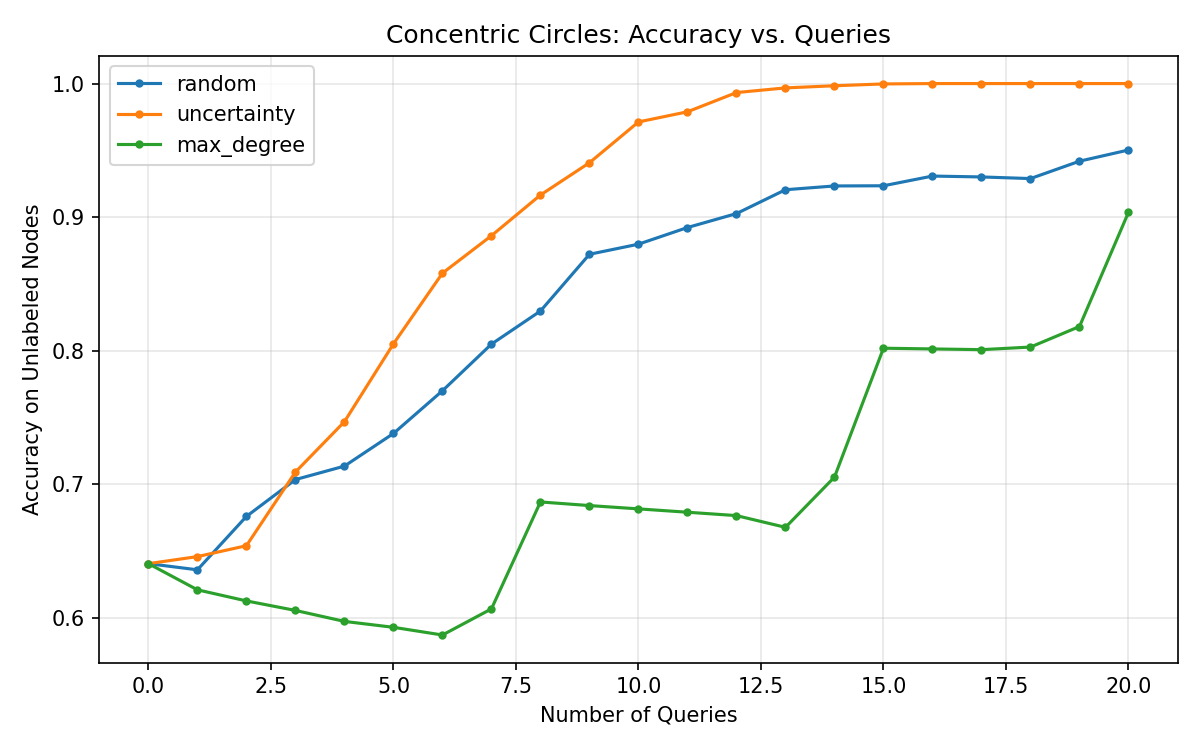
\includegraphics[width=0.85\textwidth]{figures/circles_results.png}
\caption{Concentric Circles: accuracy vs.\ number of queries. The gap between strategies is even more pronounced here. Uncertainty sampling reaches 100\% accuracy by query 12. Maximum degree selection actually \textit{decreases} in accuracy during early iterations before recovering, because the highest-degree nodes sit in the densest part of each ring --- far from the radial decision boundary --- and labeling them provides little useful information.}
\label{fig:circles}
\end{figure}

\begin{figure}[H]
\centering
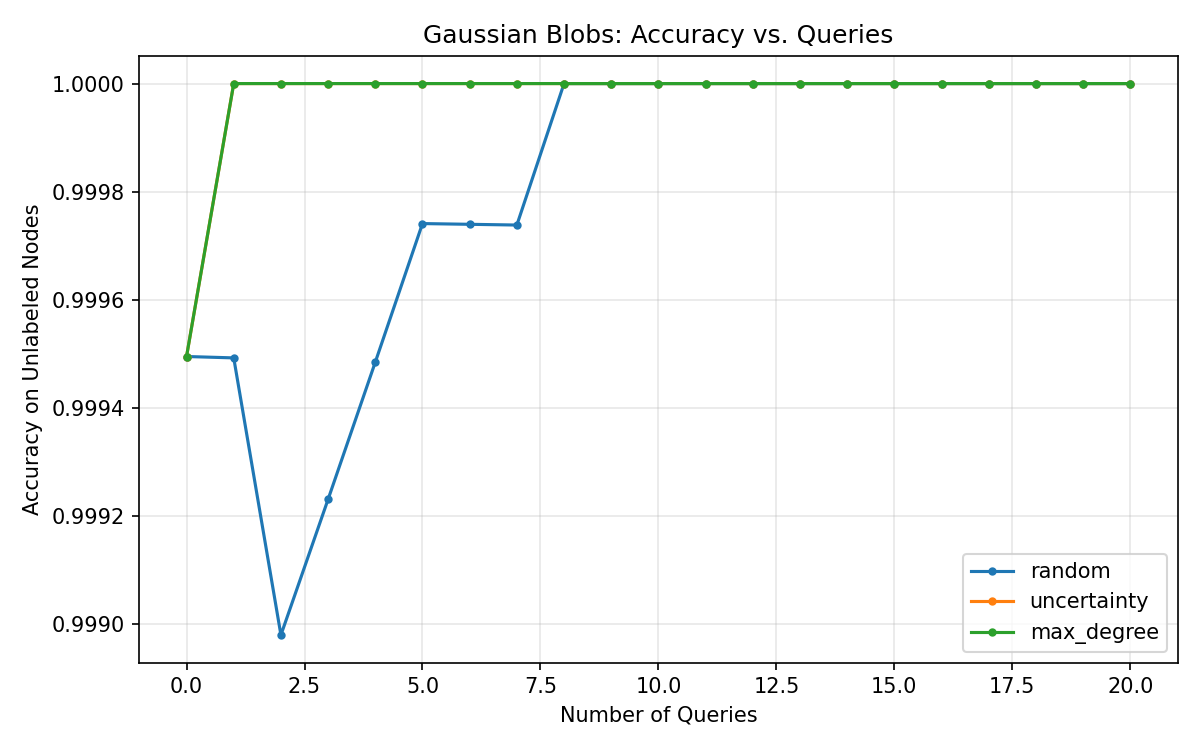
\includegraphics[width=0.85\textwidth]{figures/blobs_results.png}
\caption{Gaussian Blobs: accuracy vs.\ number of queries. All strategies achieve near-perfect accuracy almost immediately. With well-separated clusters, GFHF classifies correctly using just the two initial seed labels, and additional queries provide negligible benefit regardless of strategy. This confirms that the implementation is correct and that strategy choice only matters when the classification problem is genuinely difficult.}
\label{fig:blobs}
\end{figure}

\textbf{Two Moons} (Figure~\ref{fig:two_moons}). Uncertainty sampling clearly outperforms both alternatives, reaching over 99\% accuracy by query 10 while random selection plateaus around 96\% and maximum degree around 94\%. The two moons dataset has a curved decision boundary, and uncertainty sampling effectively targets nodes along this boundary where the harmonic function value is close to 0.5. Maximum degree selection, by contrast, picks well-connected nodes that tend to be deep inside one of the moons --- regions already classified correctly --- yielding little new information.

\textbf{Concentric Circles} (Figure~\ref{fig:circles}). The differences are even starker. Uncertainty sampling reaches perfect accuracy by query 12. Maximum degree not only fails to keep pace but actually performs \textit{worse} than the initial accuracy during early iterations. The highest-degree nodes in concentric circles lie in the densest part of each ring, far from the radial boundary between the inner and outer circles. Labeling these nodes wastes budget on regions where GFHF already propagates labels effectively.

\textbf{Gaussian Blobs} (Figure~\ref{fig:blobs}). All strategies converge to 100\% accuracy almost immediately. With well-separated Gaussian clusters, the $k$-nearest-neighbor graph has strong within-cluster connections and near-zero between-cluster connections. GFHF correctly classifies virtually all nodes with just the two initial seed labels, making additional queries largely redundant regardless of which strategy is used.

\subsection{Impact of Label Noise}

Table~\ref{tab:noise_summary} and Figure~\ref{fig:noise} show how all three strategies degrade under increasing label noise on the two moons dataset.

\begin{table}[ht]
\centering
\begin{tabular}{lccc}
\hline
\textbf{Noise Rate} & \textbf{Random} & \textbf{Uncertainty} & \textbf{Max Degree} \\
\hline
0\%  & 95.14\% & \textbf{99.61\%} & 93.74\% \\
5\%  & 93.31\% & \textbf{98.82\%} & 91.85\% \\
10\% & 91.12\% & \textbf{96.85\%} & 89.89\% \\
20\% & 85.39\% & \textbf{94.41\%} & 85.14\% \\
\hline
\end{tabular}
\caption{Mean classification accuracy after 20 queries on the Two Moons dataset under varying noise rates, averaged over 20 trials.}
\label{tab:noise_summary}
\end{table}

\begin{figure}[H]
\centering
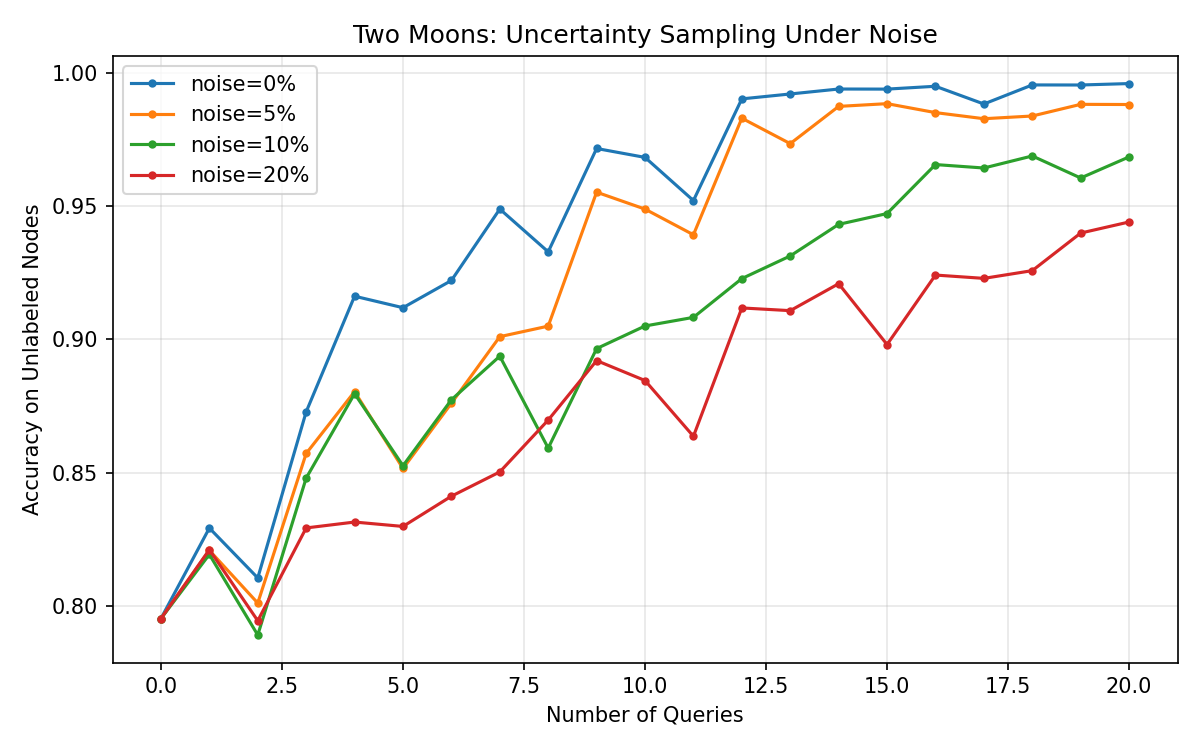
\includegraphics[width=0.85\textwidth]{figures/noise_comparison.png}
\caption{Two Moons: uncertainty sampling under increasing noise rates. At 0\% noise, accuracy reaches 99.6\% after 20 queries. At 20\% noise, accuracy still reaches 94.4\%, but convergence is slower and the curve is less stable. This demonstrates that uncertainty sampling degrades gracefully under noise rather than failing catastrophically.}
\label{fig:noise}
\end{figure}

Several observations emerge from the noise experiments. First, uncertainty sampling maintains its advantage over the other strategies at every noise level tested. Even at 20\% noise --- where one in five queried labels is incorrect --- uncertainty sampling achieves 94.41\%, compared to 85.39\% for random and 85.14\% for maximum degree.

Second, the degradation is gradual rather than catastrophic. Moving from 0\% to 20\% noise reduces uncertainty sampling's final accuracy by approximately 5 percentage points (from 99.61\% to 94.41\%), while random selection loses nearly 10 percentage points (from 95.14\% to 85.39\%). This suggests that uncertainty sampling is not only more accurate but also more robust to label noise.

Third, incorrect labels are particularly damaging when they land on structurally important nodes. Because uncertainty sampling selects nodes at the decision boundary, a flipped label at the boundary can mislead predictions for nearby nodes on both sides. Despite this vulnerability, uncertainty sampling still outperforms the alternatives, indicating that the benefit of targeting informative nodes outweighs the risk of occasional label corruption.


\section{Conclusion}

This project evaluated how active learning query strategies affect the performance of graph-based label propagation using the Gaussian Fields and Harmonic Functions (GFHF) method. Three strategies were compared --- random selection, uncertainty sampling, and maximum degree selection --- across three synthetic datasets and under four noise levels.

The results clearly demonstrate that the choice of which nodes to label matters significantly. Uncertainty sampling consistently outperformed both random selection and maximum degree selection across all datasets and noise conditions. On the two moons dataset, uncertainty sampling reached 99.61\% accuracy after 20 queries, compared to 95.14\% for random and 93.74\% for maximum degree. On concentric circles, uncertainty sampling achieved perfect classification while maximum degree struggled, highlighting that structural importance (high degree) does not necessarily correlate with informativeness for label propagation.

Maximum degree selection performed worse than random selection on every dataset with a non-trivial decision boundary. This is a meaningful finding: the most connected nodes are not the most useful nodes to label. High-degree nodes tend to sit in dense cluster interiors where GFHF already propagates labels effectively. The most valuable nodes to label are those at the boundary between classes, where the harmonic function is most uncertain.

The noise experiments confirmed that uncertainty sampling degrades gracefully under imperfect labeling. Even at a 20\% noise rate, uncertainty sampling maintained a clear advantage over the alternatives, losing approximately 5 percentage points compared to nearly 10 for random selection. This robustness is encouraging for real-world applications where label quality cannot be guaranteed.

Several directions remain for future work. First, implementing Class Mass Normalization (CMN) could improve performance on imbalanced datasets where the simple 0.5 threshold produces biased predictions. Second, more sophisticated noise models --- such as the multi-labeler framework of Fang et al.\ (2014) --- could better simulate realistic crowdsourcing scenarios. Third, combining uncertainty with structural information, as in Bilgic et al.'s ALFNET algorithm, may yield strategies that outperform either approach alone. Finally, evaluating on real-world graph datasets such as citation networks would test whether these findings generalize beyond synthetic settings.


\begin{thebibliography}{9}

\bibitem{Zhu2003}
X.~Zhu, Z.~Ghahramani, and J.~D.~Lafferty.
\newblock Semi-supervised learning using {G}aussian fields and harmonic functions.
\newblock In \emph{Proceedings of the 20th International Conference on Machine Learning (ICML-03)}, pages 912--919, 2003.

\bibitem{Bilgic2010}
M.~Bilgic, L.~Mihalkova, and L.~Getoor.
\newblock Active learning for networked data.
\newblock In \emph{Proceedings of the 27th International Conference on Machine Learning (ICML-10)}, 2010.

\bibitem{Fang2014}
M.~Fang, J.~Yin, and D.~Tao.
\newblock Active learning for crowdsourcing using knowledge transfer.
\newblock In \emph{Proceedings of the AAAI Conference on Artificial Intelligence}, volume~28, 2014.

\bibitem{Lewis1994}
D.~Lewis and W.~Gale.
\newblock A sequential algorithm for training text classifiers.
\newblock In \emph{Proceedings of SIGIR}, 1994.

\end{thebibliography}

\end{document}